\section{Comparative Study of Container Management Tools}
\label{sec:comparison}
The tools  discussed in this paper supports most of the basic features of a container orchestration tools. However, these tools differ from each other by supporting additional other features, in terms of their compatibility, easy of use and extensibility. 

Apache's Mesos has  been used in large production environment supporting tens of thousands of nodes. It is designed for big clusters. Hence, it is complicated to use Mesos in a small cluster. However, CoreOS's Fleet limitation to hundreds of nodes makes it more suitable for small scale cluster. With recent development, Kubernetes and Docker's Swarm supports a cluster of thousand nodes too. 

Due to built on the several years of experience in production environment, Kubernetes is most versatile in terms of various functionalities. For example, it supports smooth rolling update with feature to rollback. With its labeling feature, it is easy to group the task. Kubernetes is also supported by many PaaS tools. Apart from Kubernetes, Swarm also supports labeling. Swarm allows tagging a node with multiple labels which allows user to put multiple and wider constraints on a container.

Service discovery feature is supported by all the discussed tools. However, Amazon's ECS requires Docker's native container link functionality to support service discovery. 

The other two basic features of a container orchestration tool, state management and scheduling, is supported by all the discussed tools.  Mesos, Swarm and ECS allow to have a third party scheduler separating the scheduling from the state management, while Kubernetes and Fleet doesn't.

Kubernetes and Mesos are the only ones that support health monitoring. This feature is made easier by Amazon's ECS because ECS handles the health monitoring itself making it automated.

High availability of the master node is only supported by Mesos, Swarm and Fleet since they allow to have multiple instances of the master node. Kubernetes and ECS doesn't have multiple instances of master node, so they don't support high availability.

CoreOS's Fleet uses etcd and extends the systemmd feature, which was designed for single host, to support a multiple nodes cluster. In Fleet's framework, each node runs fleet daemon so any node can be a master node. So, instead of having multiple instances of master nodes, fleet implements distributed master node. 

Since Fleet is a lower level software, handling all the features is not as smooth compared to other tools for example: scheduling based on utilization. It is more suitable to run another orchestration tool on top of CoreOS's Fleet.

Mesos, fleet and ECS allows to run other orchestration tools on top of them. For example, we can run kubernetes on top of coreOs's fleet. However, Kubernetes and Swarm doesn't support this feature.

Feature of having a persistent data on a node which is shared across the containers is supported by all the mentioned tools.

In terms of ease of use, Docker's Swarm is on the top due to its compatibility with Docker's API. Containers can launched with simple Docker command. Being the native tool of a Docker, it is easily compatible with other Docker tools. However, any limitation of Docker APIs are obviously the limitations of Docker's Swarm.

Docker Swarm is also very lightweight compared to other tools except CoreOS's fleet which is a lightweight linux distribution without having any package manager. The requirement to prescale the cluster in Amazon's ECS is its only disadvantage in terms of easy of use.

Except for Swarm, container's recovery is supported by kubernetes, Mesos and ECS.

To summarize, all these tools supports the basic features of a container orchestration tool. While Docker's Swarm compatibility with Docker's API makes it easier to use, Kubernetes's robustness and making the faults not affecting availability is well tested as Kubernetes is based on 15 years of experience in production environment. Being lower level software, CoreOS's Fleet is more suitable for a small cluster and running other tools on top of it. If your application or services are already using AWS features, Amazon's ECS is the best choice. Although Mesos was developed before the sudden growth in use of containers, it supports cluster of containerized applications and if the cluster has tens of thousands of nodes, then Mesos is the best choice.

Table 1 summarizes the comparison of various features of these five container management tools discussed in this section.

\begin{figure*}
\centering
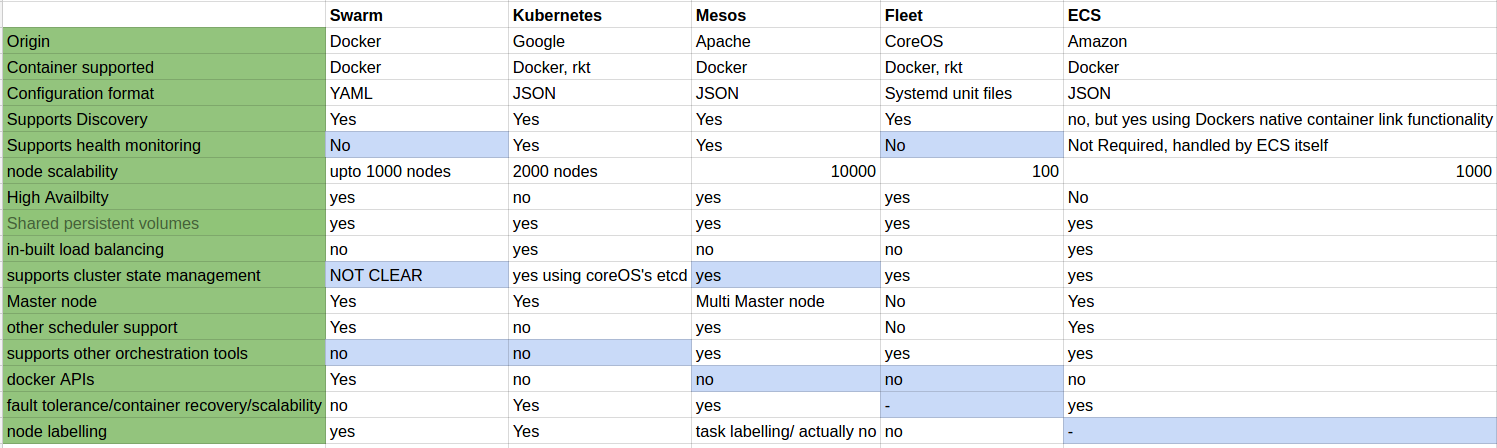
\includegraphics[width=\textwidth]{./fig/comparison}
\caption{Comparison Table}
\label{fig:comparison}
\end{figure*}


\begin{table*}[ht]
\caption{Comparison of various features}
\centering
\begin{tabular}{p{0.14\linewidth}p{0.14\linewidth}p{0.14\linewidth}p{0.14\linewidth}p{0.14\linewidth}p{0.14\linewidth}}
\hline
Features & Swarm & Kubernetes & Mesos & Fleet & ECS\\
\hline
Origin & Docker & Google & Apache &	CoreOS & Amazon\\

Container supported & Docker & Docker, rkt & Docker &	Docker, rkt & Docker\\

Configuration format	& YAML &	JSON & JSON & Systemd unit files & JSON\\

Supports Discovery  & yes & yes & yes & yes & no\raise0.5ex\hbox{1}\\

Supports health monitoring & no & yes & yes & no & no\raise0.5ex\hbox{2}\\

node scalability	& upto 1000 nodes & 2000 nodes & 10000 & 100 & 1000\\

High Availbilty	& yes &	no & yes &	yes &	no\\

Shared persistent volumes & yes & yes & yes & yes & yes\\

in-built load balancing & no &	yes &	no &	no &	yes\\

supports cluster state management & NOT CLEAR & yes\raise0.5ex\hbox{3} & yes & yes & yes\\

Master node	 & yes & yes & Multi Master node &	no &	yes\\

other scheduler support & yes & no & yes & no & Yes\\

supports other orchestration tools	 & no  & no &	yes &	yes &	yes\\

docker APIs	 & yes & no &	no & no & no\\

fault tolerance/container recovery/scalability  & no & yes & yes & - & yes\\

node labelling & yes & yes & no\raise0.5ex\hbox{4} & no & -\\
\hline
\end{tabular}
\\
1. yes, using Dockers native container link functionality\\
2. Not required as it is handled by ECS itself\\
3. using coreOS's etcd\\
4. But task labelling: yes
\end{table*}

